\section{\LangPPCF{}}

The textbook presentation of \LangPCF{} gives us the means of executing computations in
parallel. We'd like to generalize the binary fork-join model we've seen so far, as well as to
examine the cost of parallel programs more closely. So far in \LangPCF{}, the notion of a value
was an expression that cannot be evaluated further. This is still the case in the parallel
formulation, but we should now be more careful on the issue of cost.

Suppose the user provides as input a long list of number literals. Any reasonable representation
of lists will represent this as a value, i.e. not provide a means of evaluating it further.
However, the value judgment is defined inductively, meaning an interpreter must still examine the
entire list and every element within it in order to conclude that it is a value. This process
incurs linear cost. Now imagine that this list is used as an argument to a function, and
substituted in several locations throughout the function body. Now the interpreter will repeatedly
evaluate this object, and the cost becomes nontrivial. The notion of value, as specified by the
dynamics, has diverged from a more desirable definition of value under parallelism:
\emph{a data element for which we need incur no additional cost}.

The solution is to utilize a \emph{modally separate} semantics.
Here, we make the claim that expressions are not values, but through the incurring of cost
may eventually compute a value. That's a powerful concept, which lets us precisely state that costs
should be attributed to expressions when they perform computation to result in values.

\clearpage

\subsection{\LangPPCF{}}

Once again, we present a user-facing language \LangPPCF{} which is friendly to program in.
Then, we give a modally-separated presentation \LangPPCFv{} that we immediately elaborate to.

\begin{figure}
  \begin{adjustbox}{tabular=LLLLLL,center}
    \TypeSort & \tau & \Coloneqq & \nattyabt                      & \nattycst                           & \code{nat} \\
              &      &           & \parrtyabt{\tau_1}{\tau_2}     & \parrtycst{\tau_1}{\tau_2}          & \code{tau1 -> tau2} \\
              &      &           & \eprodtyabt{n}{\many{;}{\tau}} & \eprodtycst{n}{\many{\epsep}{\tau}} & \code{tau1 @ ... @ taun} \\
              &      &           & \lprodtyabt{n}{\many{;}{\tau}} & \lprodtycst{n}{\many{\lpsep}{\tau}} & \code{\{ tau1 \& ... \& taun \}} \\
              &      &           & \seqtyabt{\tau}                & \seqtycst{\tau}                     & \code{tau seq} \\
              &      &           & \gentyabt{\tau}                & \gentycst{\tau}                     & \code{tau gen} \\
    \ExprSort & e    & \Coloneqq & x                                     & x                                     & \code{x}  \\
              &      &           & \letbeabt{e_1}{x}{e_2}                & \letbecst{e_1}{x}{e_2}                & \code{let x = e1 in e2} \\
              &      &           & \numabt{n}                            & n                                     & \code{n} \\
              &      &           & \primexabt{\odot}{e_1}{e_2}           & \primexcst{\odot}{e_1}{e_2}           & \code[mathescape=true]{e1 $\ \odot\ $ e2} \\
              &      &           & \ifzabt{e}{e_0}{x}{e_1}               & \ifzcst{e}{e_0}{x}{e_1}               & \code{ifz e \{ z => e0 | s(x) \ => e1 \}} \\
              &      &           & \funabt{\tau_1}{\tau_2}{f}{x}{e}      & \funcst{\tau_1}{\tau_2}{f}{x}{e}      & \code{fun f (x : tau1) \ : tau2 is e} \\
              &      &           & \lamabt{\tau}{x}{e}                   & \lamcst{\tau}{x}{e}                   & \code{fn (x : tau) \ => e} \\
              &      &           & \appabt{e}{e_1}                       & \appcst{e}{e_1}                       & \code{e e1} \\
              &      &           & \splitabt{n}{e}{\many{,}{x}}{e'}      & \splitcst{n}{e}{\many{,}{x}}{e'}      & \code{split e as x1, ..., xn in e'} \\
              &      &           & \ltupabt{n}{\many{;}{e}}              & \ltupcst{n}{\many{\ltsep}{e}}         & \code{\{ e1 \& ... \& en \}} \\
              &      &           & \parabt{e}                            & \parcst{e}                            & \code{par e} \\
              &      &           & \lenabt{e}                            & \lencst{e}                            & \code{|e|} \\
              &      &           & \subabt{e}{e_\text{index}}            & \subcst{e}{e_\text{index}}            & \code{e[eindex]} \\
              &      &           & \genabt{\tau}{e_\text{length}}{i}{e}  & \gencst{\tau}{e_\text{length}}{i}{e}  & \code{gen\{tau\}[elength] with i in e} \\
              &      &           & \tababt{e}                            & \tabcst{e}                            & \code{tab e}
  \end{adjustbox}
  \caption{\LangPPCF{} Grammar}
  \label{fig:ppcf}
\end{figure}

\LangPPCF{} will inherit a \emph{by-value} interpretation of \LangPCF{}, extended with types that enable parallel computation.
The syntax of \LangPPCF{} is given in \Cref{fig:ppcf}.

This language has \LangPCF{}'s natural and function types, along with two new product types, one eager and one lazy.
Zero or more expressions may be suspended as values using lazy products.

Rather than building natural numbers explicitly via zero and successor, we provide a numeric literal primitive.
Furthermore, we provide a collection of primitive operations on natural numbers, where $\odot$ ranges over $+, -, \times, \div, \le$.
For simplicity, division by zero returns zero.
Additionally, we define $e_1 \le e_2$ as $1$ if $e_1$ is less than or equal to $e_2$, or $0$ otherwise.

\subsection{\LangPPCFv{}}

The grammar of \LangPPCFv{} is given in \Cref{fig:ppcfv}.

We include internal forms $\etupabt{n}{\many{;}{v}}$ and $\seqabt{\tau}{n}{\many{,}{v}}$ which cannot be directly written by the programmer.
They can still be manipulated, but they will only show up as variables.
Their introduction forms are the elimination forms of lazy tuples and generators, respectively.

\begin{figure}
  \begin{adjustbox}{tabular=LLLLLl,center}
    \TypeSort & \tau & \Coloneqq & \comptyabt{\tau}               & \comptycst{\tau}                    & computation \\
              &      &           & \nattyabt                      & \nattycst                           & naturals \\
              &      &           & \parrtyabt{\tau_1}{\tau_2}     & \parrtycst{\tau_1}{\tau_2}          & partial functions \\
              &      &           & \eprodtyabt{n}{\many{;}{\tau}} & \eprodtycst{n}{\many{\epsep}{\tau}} & eager products \\
              &      &           & \lprodtyabt{n}{\many{;}{\tau}} & \lprodtycst{n}{\many{\lpsep}{\tau}} & lazy products \\
              &      &           & \seqtyabt{\tau}                & \seqtycst{\tau}                     & sequences \\
              &      &           & \gentyabt{\tau}                & \gentycst{\tau}                     & generators \\
    \ValueSort & v & \Coloneqq & x                                & x                                & variable  \\
               &   &           & \compabt{e}                      & \compcst{e}                      & suspended computation \\
               &   &           & \numabt{n}                       & n                                & numeric literal \\
               &   &           & \funabt{\tau_1}{\tau_2}{f}{x}{e} & \funcst{\tau_1}{\tau_2}{f}{x}{e} & recursive function \\
               &   &           & \lamabt{\tau}{x}{e}              & \lamcst{\tau}{x}{e}              & non-recursive function \\
               &   &           & \etupabt{n}{\many{;}{v}}         & \etupcst{n}{\many{\tsep}{v}}     & eager tuple \\
               &   &           & \ltupabt{n}{\many{;}{e}}         & \ltupcst{n}{\many{\ltsep}{e}}    & lazy tuple \\
               &   &           & \seqabt{\tau}{n}{\many{,}{v}}    & \seqcst{\tau}{n}{\many{,}{v}}    & sequence \\
               &   &           & \genabt{\tau}{v}{i}{e}           & \gencst{\tau}{v}{i}{e}           & sequence generator \\
    \ExprSort & e & \Coloneqq & \retabt{v}                      & \retcst{v}                      & trivial computation  \\
              &   &           & \bindabt{v}{x}{e}               & \bindcst{v}{x}{e}               & sequential evaluation \\
              &   &           & \primexabt{\odot}{v_1}{v_2}     & \primexcst{\odot}{v_1}{v_2}     & primitive arithmetic operation \\
              &   &           & \ifzabt{v}{e_0}{x}{e_1}         & \ifzcst{v}{e_0}{x}{e_1}         & zero test \\
              &   &           & \appabt{v}{v_1}                 & \appcst{v}{v_1}                 & function application \\
              &   &           & \splitabt{n}{v}{\many{,}{x}}{e} & \splitcst{n}{v}{\many{,}{x}}{e} & tuple split \\
              &   &           & \parabt{v}                      & \parcst{v}                      & parallel evaluation \\
              &   &           & \lenabt{v}                      & \lencst{v}                      & sequence length \\
              &   &           & \subabt{v}{v_\text{index}}      & \subcst{v}{v_\text{index}}      & sequence subscript \\
              &   &           & \tababt{v}                      & \tabcst{v}                      & parallel sequence tabulation \\
  \end{adjustbox}
  \caption{\LangPPCFv{} Grammar}
  \label{fig:ppcfv}
\end{figure}

\subsection{Statics}

Similar to \LangKPCFv{}, we will have two judgments in our static semantics: one for values and one for computations.

\fbox{$\typeJC{v}{\tau}$}
\begin{mathpar}
  \inferrule
    {\strut}
    {\typeJ{\ctx, \IsOf{x}{\tau}}{x}{\tau}}

  \inferrule
    {\eTypeJC{e}{\tau}}
    {\typeJC{\compabt{e}}{\comptycst{\tau}}}

  \inferrule
    {\strut}
    {\typeJC{\numabt{n}}{\nattyabt}}

  \inferrule
    {\eTypeJ{\ctx, \IsOf{f}{\parrtycst{\tau_1}{\tau_2}, \IsOf{x}{\tau_1}}}{e}{\tau_2}}
    {\typeJC{\funabt{\tau_1}{\tau_2}{f}{x}{e}}{\parrtycst{\tau_1}{\tau_2}}}

  \inferrule
    {\eTypeJ{\ctx, \IsOf{x}{\tau_1}}{e}{\tau_2}}
    {\typeJC{\lamabt{\tau_1}{x}{e}}{\parrtycst{\tau_1}{\tau_2}}}

  \inferrule
    {\typeJC{v_1}{\tau_1} \\ \ldots \\ \typeJC{v_n}{\tau_n}}
    {\typeJC{\etupabt{n}{\many{\tsep}{v}}}{\eprodtycst{n}{\many{\epsep}{\tau}}}}

  \inferrule
    {\eTypeJC{e_1}{\tau_1} \\ \ldots \\ \eTypeJC{e_n}{\tau_n}}
    {\typeJC{\ltupabt{n}{\many{\ltsep}{e}}}{\lprodtycst{n}{\many{\lpsep}{\tau}}}}

  \inferrule
    {\typeJC{v_1}{\tau} \\ \ldots \\ \typeJC{v_n}{\tau}}
    {\typeJC{\seqabt{\tau}{n}{\many{,}{v}}}{\seqtycst{\tau}}}

  \inferrule
    {\typeJC{v}{\nattycst} \\ \eTypeJ{\ctx, \IsOf{i}{\nattycst}}{e}{\tau}}
    {\typeJC{\genabt{\tau}{v}{i}{e}}{\gentycst{\tau}}}
\end{mathpar}

The value typing judgment is woven into the expression typing judgment.
Here, the most interesting thing is that lazy tuples have lazy product type and eager
tuples have eager product type. Likewise, sequences have sequence type and generators have
generator type.

\fbox{$\eTypeJC{e}{\tau}$}
\begin{mathpar}
  \inferrule
    {\typeJC{v}{\tau}}
    {\eTypeJC{\retabt{v}}{\tau}}

  \inferrule
    {\typeJC{v}{\comptycst{\tau_1}} \\ \eTypeJ{\ctx, \IsOf{x}{\tau_1}}{e}{\tau_2}}
    {\eTypeJC{\bindabt{v}{x}{e}}{\tau_2}}

  \inferrule
    {\typeJC{v_1}{\nattycst} \\ \typeJC{v_2}{\nattycst}}
    {\eTypeJC{\primexabt{\odot}{v_1}{v_2}}{\nattycst}}

  \inferrule
    {\typeJC{v}{\nattyabt} \\ \eTypeJC{e_0}{\tau} \\ \eTypeJ{\ctx, \IsOf{x}{\nattyabt}}{e_1}{\tau}}
    {\eTypeJC{\ifzabt{v}{e_0}{x}{e_1}}{\tau}}

  \inferrule
    {\typeJC{v}{\parrtycst{\tau_1}{\tau_2}} \\ \typeJC{v_1}{\tau_1}}
    {\eTypeJC{\appabt{v}{v_1}}{\tau_2}}

  \inferrule
    {\typeJC{v}{\eprodtycst{n}{\many{\epsep}{\tau}}} \\ \eTypeJ{\ctx, \IsOf{x_1}{\tau_1}, \ldots, \IsOf{x_n}{\tau_n}}{e}{\tau}}
    {\eTypeJC{\splitabt{n}{v}{\many{,}{x}}{e}}{\tau}}

  \inferrule
    {\typeJC{v}{\lprodtycst{n}{\many{\lpsep}{\tau}}}}
    {\eTypeJC{\parabt{v}}{\eprodtycst{n}{\many{\epsep}{\tau}}}}

  \inferrule
    {\typeJC{v}{\seqtycst{\tau}}}
    {\eTypeJC{\lenabt{v}}{\nattycst}}

  \inferrule
    {\typeJC{v}{\seqtycst{\tau}} \\ \typeJC{v_\text{index}}{\nattycst}}
    {\eTypeJC{\subabt{v}{v_\text{index}}}{\tau}}

  \inferrule
    {\typeJC{v}{\gentycst{\tau}}}
    {\eTypeJC{\tababt{v}}{\seqtycst{\tau}}}
\end{mathpar}

Most of the constructs are familiar and behave as expected.
The tuple split construct pattern matches an eager tuple against as many variables as there are elements in the tuple.
Finally, the parallel evaluation construct is simultaneously an elimination for the lazy tuple and an introduction for the eager tuple.
Likewise for the parallel sequence evaluation, which eliminates generators and introduces sequences.

Why do we call the lazy tuple lazy? Values of lazy product type hold $n$ expressions (computations)
suspended, able to be forced later. When we are ready to evaluate each element of the tuple in
parallel, we may force its evaluation using the $\parcst{v}$ construct. Each independent element
is evaluated, and an eager tuple is made available containing the results of the computations.

We can express computations using tuples with sequences as well, presenting the difference between
static parallelism and dynamic parallelism. Though dynamic parallelism with sequences is more flexible,
it is slightly deficient in its safety guarantees and can potentially be more difficult to schedule at runtime.

\subsection{Evaluation Dynamics}

Though we will not implement \LangPPCFv{} using evaluation dynamics, it is a very
useful tool for understanding how the language evaluates, and which components are evaluated
in parallel.

The evaluation dynamics are defined in terms of the judgment $\CostEvalsTo{e}{v}{c}$, where
the cost $c$ is the abstract cost of the operation. We use $\seqcomp$ to
denote sequential composition and $\parcomp$ to denote parallel composition.
\begin{mathpar}
  \inferrule
    {\strut}
    {\CostEvalsTo{\retabt{v}}{v}{\zerocost}}

  \inferrule
    {\CostEvalsTo{e_1}{v_1}{c_1} \\ \CostEvalsTo{\Subst{v_1}{x}{e_2}}{v_2}{c_2}}
    {\CostEvalsTo{\bindabt{\compabt{e_1}}{x}{e_2}}{v_2}{c_1 \seqcomp \unitcost \seqcomp c_2}}

  \inferrule
    {n_1 \odot n_2 = n}
    {\CostEvalsTo{\primexabt{\odot}{\numabt{n_1}}{\numabt{n_2}}}{\numabt{n}}{\unitcost}}

  \inferrule
    {\CostEvalsTo{e_0}{v}{c}}
    {\CostEvalsTo{\ifzabt{\numabt{0}}{e_0}{x}{e_1}}{v}{\unitcost \seqcomp c}}

  \inferrule
    {\CostEvalsTo{\Subst{\numabt{n}}{x}{e_1}}{v}{c}}
    {\CostEvalsTo{\ifzabt{\numabt{n + 1}}{e_0}{x}{e_1}}{v}{\unitcost \seqcomp c}}

  \inferrule
    {\CostEvalsTo{\Subst{\funabt{\tau_1}{\tau_2}{f}{x}{e},v_1}{f,x}{e}}{v}{c}}
    {\CostEvalsTo{\appabt{\funabt{\tau_1}{\tau_2}{f}{x}{e}}{v_1}}{v}{\unitcost \seqcomp c}}

  \inferrule
    {\CostEvalsTo{\Subst{v_1}{x}{e}}{v}{c}}
    {\CostEvalsTo{\appabt{\lamabt{\tau}{x}{e}}{v_1}}{v}{\unitcost \seqcomp c}}

  \inferrule
    {\CostEvalsTo{\Subst{\many{,}{v}}{\many{,}{x}}{e}}{v}{c}}
    {\CostEvalsTo{\splitabt{n}{\etupcst{n}{\many{\tsep}{v}}}{\many{,}{x}}{e}}{v}{\unitcost \seqcomp c}}

  \inferrule
    {\CostEvalsTo{e_1}{v_1}{c_1} \\ \ldots \\ \CostEvalsTo{e_n}{v_n}{c_n}}
    {\CostEvalsTo{\parabt{\ltupcst{n}{\many{\ltsep}{e}}}}{\etupcst{n}{\many{\tsep}{v}}}{(\many{\parcomp}{c}) \seqcomp \unitcost}}

  \inferrule
    {\strut}
    {\CostEvalsTo{\lenabt{\seqcst{\tau}{n}{\many{,}{v}}}}{\numabt{n}}{\unitcost}}

  \inferrule
    {i < n}
    {\CostEvalsTo{\subcst{\seqcst{\tau}{n}{\manyz{,}{v}}}{\numabt{i}}}{v_i}{\unitcost}}

  \inferrule
    {0 \le n \\ \CostEvalsTo{[\numabt{0}/i]e}{v_1}{c_1} \\ \ldots \\ \CostEvalsTo{[\numabt{n-1}/i]e}{v_n}{c_n}}
    {\CostEvalsTo{\tababt{\gencst{\tau}{\numabt{n}}{i}{e}}}{\seqcst{\tau}{n}{\many{,}{v}}}{(\many{\parcomp}{c}) \seqcomp \unitcost}}
\end{mathpar}

Evaluation semantics precisely describe ``what'' the expressions should do, but not ``how'' to do
so in parallel. For that, we use a more involved structural dynamics. As you saw, it is possible to
relate the evaluation semantics to the structural semantics by proving their equivalence regarding
cost assignments, but here we will take their conceptual equivalence for granted.

\subsubsection{Cost Graphs}

\textit{Cost graphs} are one notion of abstract cost we may wish to consider.
Cost graphs are defined inductively as follows:

\[
  \begin{array}{r c l l}
    c & \Coloneqq & \zerocost          & \text{zero cost} \\
      &           & \unitcost          & \text{unit cost} \\
      &           & \parcost{c_1}{c_2} & \text{parallel combination} \\
      &           & \seqcost{c_1}{c_2} & \text{sequential combination} \\
  \end{array}
\]

Rather than working with the textual representation of cost graphs,
we can draw them out in true \textit{graph}ical fashion.
Cost graphs can be visually represented as shown in \Cref{fig:cost-graphs},
where source nodes are labelled with $s$ and sink nodes are labelled with $t$.

\begin{figure}
  \centering
  \begin{subfigure}{0.2\textwidth}
    \centering
    \begin{tikzpicture}
      \node[shape=circle] (B) at (0,0) {};
      \node[shape=circle,draw=black] (A) at (0,1.5) {$s$/$t$};
      \node[shape=circle] (C) at (0,3) {};
    \end{tikzpicture}
    \caption{Cost graph of $\zerocost$}
  \end{subfigure}
  \begin{subfigure}{0.2\textwidth}
    \centering
    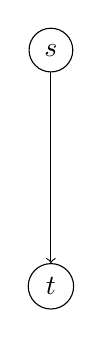
\begin{tikzpicture}
        \node[shape=circle,draw=black] (A) at (0,3) {$s$};
        \node[shape=circle,draw=black] (B) at (0,0) {$t$};

        \path [->] (A) edge node[left] {} (B);
    \end{tikzpicture}
    \caption{Cost graph of $\unitcost$}
  \end{subfigure}
  \begin{subfigure}{0.25\textwidth}
    \centering
    \begin{tikzpicture}
        \node[shape=circle,draw=black] (S) at (0,5) {$s_1, s_2$};
        \node[diamond,draw=black,minimum size=2cm] (C1) at (-1.5,2.5) {$c_1$};
        \node[diamond,draw=black,minimum size=2cm] (C2) at (1.5,2.5) {$c_2$};
        \node[shape=circle,draw=black] (T) at (0,0) {$t_1, t_2$};

        \path [->] (S) edge node[left] {} (C1.north);
        \path [->] (S) edge node[left] {} (C2.north);
        \path [->] (C1.south) edge node[left] {} (T);
        \path [->] (C2.south) edge node[left] {} (T);
    \end{tikzpicture}
    \caption{Cost graph of $\parcost{c_1}{c_2}$}
  \end{subfigure}
  \begin{subfigure}{0.25\textwidth}
    \centering
    \begin{tikzpicture}
      \node[shape=circle,draw=black] (S) at (0,6) {$s_1$};
      \node[diamond,draw=black] (C1) at (0,4.5) {$c_1$};
      \node[shape=circle,draw=black] (ST) at (0,3) {$t_1,s_2$};
      \node[diamond,draw=black] (C2) at (0,1.5) {$c_2$};
      \node[shape=circle,draw=black] (T) at (0,0) {$t_2$};

      \path [->] (S.south) edge node[left] {} (C1.north);
      \path [->] (C1.south) edge node[left] {} (ST.north);
      \path [->] (ST.south) edge node[left] {} (C2.north);
      \path [->] (C2.south) edge node[left] {} (T.north);
    \end{tikzpicture}
    \caption{Cost graph of $\seqcost{c_1}{c_2}$}
  \end{subfigure}
  \caption{Visual representations of primitive cost graphs}
  \label{fig:cost-graphs}
\end{figure}

Some sample cost graphs are depicted in \Cref{fig:cost-graph-ex}.
\begin{figure}
  \centering
  \begin{subfigure}[b]{0.2\textwidth}
    \centering
    \begin{tikzcd}
      \bullet \\
      \bullet \\
      \bullet
      \arrow[curve={height=12pt}, from=1-1, to=2-1]
      \arrow[curve={height=-12pt}, from=1-1, to=2-1]
      \arrow[from=2-1, to=3-1]
    \end{tikzcd}
    \caption{$\seqcost{\cdparens{\parcost{\unitcost}{\unitcost}}}{\unitcost}$}
  \end{subfigure}
  \begin{subfigure}[b]{0.2\textwidth}
    \centering
    \begin{tikzcd}
      \bullet \\
      \bullet \\
      \bullet
      \arrow[curve={height=12pt}, from=2-1, to=3-1]
      \arrow[curve={height=-12pt}, from=2-1, to=3-1]
      \arrow[from=2-1, to=3-1]
      \arrow[from=1-1, to=2-1]
    \end{tikzcd}
    \caption{$\seqcost{\unitcost}{\cdparens{\parcost{\unitcost}{\parcost{\unitcost}{\unitcost}}}}$}
  \end{subfigure}
  \begin{subfigure}[b]{0.2\textwidth}
    \centering
    \begin{tikzcd}
      \bullet \\
      & \bullet \\
      \bullet
      \arrow[from=1-1, to=3-1]
      \arrow[from=1-1, to=2-2]
      \arrow[from=2-2, to=3-1]
    \end{tikzcd}
    \caption{$\parcost{\unitcost}{\cdparens{\seqcost{\unitcost}{\unitcost}}}$}
  \end{subfigure}
  \begin{subfigure}[b]{0.3\textwidth}
    \centering
    \begin{tikzcd}
      & \bullet \\
      && \bullet \\
      \bullet && \bullet \\
      & \bullet
      \arrow[from=1-2, to=2-3]
      \arrow[from=1-2, to=4-2]
      \arrow[from=2-3, to=3-3]
      \arrow[from=3-3, to=4-2]
      \arrow[from=1-2, to=3-1]
      \arrow[from=3-1, to=4-2]
    \end{tikzcd}
    \caption{$\parcost{\cdparens{\seqcost{\unitcost}{\unitcost}}}{\parcost{\unitcost}{\cdparens{\seqcost{\unitcost}{\seqcost{\unitcost}{\unitcost}}}}}$}
  \end{subfigure}
  \caption{Sample cost graphs}
  \label{fig:cost-graph-ex}
\end{figure}

In this section, we will be exploring cost graphs by drawing cost
graphs associated with the \LangPPCFv{} expressions below.

\clearpage

\task{15} Draw the cost graphs of the following \LangPPCFv{} expressions:

\begin{enumerate}
  \item
    \begin{align*}
      &\parcst{\ltupcst{}{ \\
      &\quad (1 + 2) \; \\
      &\quad \& \; \ifzcst{3}{\retcst{1}}{x}{\retcst{2}} \; \\
      &\quad \& \; \bindabt{\compcst{\tababt{\genabt{\nattycst}{3}{x}{x + 1}}}}{y}{\lencst{y}} \\
      &}}
    \end{align*}

  \item
    $\bindabt
      {\compcst{e_1}}
      {z}
      {
        \bindabt
          {\compcst{e_2}}
          {n}
          {e_3}
      }$

    where we define:
    \begin{align*}
      e_1 &= \parcst{\ltupcst{}{(1 + 2) \; \& \; (6 - 4)}} \\
      e_2 &= \splitabt{2}{z}{x, y}{x + y} \\
      e_3 &= \tababt{\genabt{\nattycst}{n}{x}{x + 1}}
    \end{align*}
  \item $\retcst{\lamcst{\nattycst}{n}{\tababt{\genabt{\nattycst}{n}{x}{x + 1}}}}$
\end{enumerate}

\solution{cost-graphs}

\subsection{Local Transitions}

The structural dynamics of \LangPPCFv{} involve two types of transitions:
local transitions, which represent the work that one processor may perform in one step on an
expression, and global transitions, which represent the work of multiple processors.
The mechanism we use to study these semantics is the $\MachP$ machine.

In the $\MachP$ machine, we introduce a new expression-like notation for join-points in the
computation.
\[ \join{\ldots}{x}{e} \]
denotes a blocked computation that depends on the result of specific computations.
This is a general mechanism to carry out a subcomputation.

We introduce a join point for a single expression when we encounter a \code{bind}:
\begin{mathpar}
  \inferrule
    {\strut}
    {
      \stepsm{
        \lstate{a}{\pbind{a}{\bindabt{\compcst{e}}{x}{e'}}}
      }{
        \lstate{a\ a_1}
        {\pbind{a}{\join{a_1}{x}{e'}}\extp{a_1}{e}}
      }
    }
\end{mathpar}
This tells the abstract machine to execute $e$ under some fresh identifier $a_1$, noting that we should continue with $\AbsABT{x}{e'}$ when $e$ finishes computing.

We may also wait to join on multiple identifiers, which is essential for stepping the parallel evaluation construct:
\begin{mathpar}
  \inferrule
    {\strut}
    {
      \stepsm{
        \lstate{a}{\pbind{a}{\parabt{\ltupcst{n}{\many{\ltsep}{e}}}}}
      }{
        \lstate{a\ a_1\ \ldots\ a_n}
        {\pbind{a}{\join{\many{,}{a}}{\many{,}{x}}{\retabt{\etupabt{n}{\many{;}{x}}}}}\extp{a_1}{e_1}\otimes\ldots\extp{a_n}{e_n}}
      }
    }
\end{mathpar}

And generators evaluate their bodies a specified number of times, substituting the index each time:
\begin{mathpar}
  \inferrule
    {0 \le n}
    {
      \stepsm{
        \lstate{a}{\pbind{a}{\tababt{\gencst{\tau}{\numabt{n}}{i}{e}}}}
      }{
        \lstate{a\ a_1\ \ldots\ a_n}
        {\pbind{a}{\join{\many{,}{a}}{\many{,}{x}}{\retabt{\seqcst{}{}{\many{,}{x}}}}}\extp{a_1}{\Subst{\numcst{0}}{i}{e}}\otimes\ldots\extp{a_n}{\Subst{\numcst{n-1}}{i}{e}}}
      }
    }
  \end{mathpar}

The elimination for a \code{join} is when all of its operands have evaluated:
\begin{mathpar}
  \inferrule
    {\strut}
    {
      \stepsm{
        \lstate{a\ a_1\ \ldots\ a_n}
        {\pbind{a}{\join{\many{,}{a}}{\many{,}{x}}{e}}\extp{a_1}{\retabt{v_1}}\otimes\ldots\extp{a_n}{\retabt{v_n}}}
      }{
        \lstate{a}{\pbind{a}{\Subst{\many{,}{v}}{\many{,}{x}}{e}}}
      }
    }
\end{mathpar}

There is no local dynamics rule for \code{ret}; it represents an expression that has been evaluated
to its fullest point. \code{ret}s are eliminated by the join points, and a total program
should eventually evaluate to $\retabt{v}$ for some value $v$. Note that this definition is slightly
different from the evaluation semantics, which take expressions to values, but is the same in
spirit.

Each other rule merely steps some expression that can evaluate:

\begin{mathpar}
  \inferrule
    {n_1 \odot n_2 = n}
    {
      \stepsl{
        \lstate{a}{\pbind{a}{\primexabt{\odot}{\numabt{n_1}}{\numabt{n_2}}}}
      }{
        \lstate{a}{\pbind{a}{\retabt{\numabt{n}}}}
      }
    }

  \inferrule
    {\strut}
    {
      \stepsl{
        \lstate{a}
        {\pbind{a}{\ifzabt{\numabt{0}}{e_0}{x}{e_1}}}
      }{
        \lstate{a}{\pbind{a}{e_0}}
      }
    }

  \inferrule
    {\strut}
    {
      \stepsl{
        \lstate{a}
        {\pbind{a}{\ifzabt{\numabt{n+1}}{e_0}{x}{e_1}}}
      }{
        \lstate{a}{\pbind{a}{\Subst{\numabt{n}}{x}{e_1}}}
      }
    }

  \inferrule
    {\strut}
    {
      \stepsl{
        \lstate{a}{\pbind{a}{\appabt{\funabt{\tau_1}{\tau_2}{f}{x}{e}}{v}}}
      }{
        \lstate{a}{\pbind{a}{\Subst{\funabt{\tau_1}{\tau_2}{f}{x}{e},v}{f,x}{e}}}
      }
    }

  \inferrule
    {\strut}
    {
      \stepsl{
        \lstate{a}{\pbind{a}{\appabt{\lamabt{\tau}{x}{e}}{v}}}
      }{
        \lstate{a}{\pbind{a}{\Subst{v}{x}{e}}}
      }
    }


  \inferrule
    {\strut}
    {
      \stepsl{
        \lstate{a}{\pbind{a}{\splitabt{n}{\etupcst{n}{\many{\tsep}{v}}}{\many{,}{x}}{e}}}
      }{
        \lstate{a}{\pbind{a}{[\many{,}{v}/\many{,}{x}]e}}
      }
    }

  \inferrule
    {\strut}
    {
      \stepsl{
        \lstate{a}{\pbind{a}{\lenabt{\seqcst{\tau}{n}{\many{,}{v}}}}}
      }{
        \lstate{a}{\pbind{a}{\retabt{\numabt{n}}}}
      }
    }

\inferrule
  {i < n}
  {
    \stepsl{
      \lstate{a}{\pbind{a}{\subcst{\seqcst{\tau}{n}{\manyz{,}{v}}}{\numabt{i}}}}
    }{
      \lstate{a}{\pbind{a}{\retabt{v_i}}}
    }
  }
\end{mathpar}

\subsubsection{Errors}

There are two kinds of errors that can occur:
\begin{enumerate}
  \item
    When an illegal subscript is taken:
    \[
      \infer{
        \errl{
          \lstate{a}{\pbind{a}{\subcst{\seqcst{\tau}{n}{\manyz{,}{v}}}{\numabt{i}}}}
        }
      }{i \ge n}
    \]

  \item
    When a generator is of negative length:
    \[
      \infer{
        \errl{
          \lstate{a}{\pbind{a}{\tababt{\gencst{\tau}{\numabt{n}}{i}{e}}}}
        }
      }{n < 0}
    \]
\end{enumerate}

Errors are propagated at join-points, and if multiple errors should result, the leftmost error
should be propagated.

\begin{mathpar}
  \infer{
    \errl{
      \lstate{\Sigma_1\ a_1\ \Sigma_2}{\mu_1 \otimes \pbind{a_1}{e_1} \otimes \mu_2}
    }
  }{\stepsl{\lstate{\Sigma_1}{\mu_1}}{\lstate{\Sigma_1}{\mu_1'}} \quad \errl{\lstate{a_1}{\pbind{a_1}{e_1}}}}
\end{mathpar}

\subsection{Global Transitions}

Each global transition represents the
simultaneous execution of one local step of computation on each of up to
$p\geq 1$ processors:
\begin{mathpar}
  \infer{
    \stepsg{
      \lstate{\sctx_1\,a_1\,\ldots\,\sctx_n\,a_n\,\sctx}
      {\pbind{a_1}{e_1} \otimes \mu_1 \otimes \ldots \otimes \pbind{a_n}{e_n} \otimes \mu_n \otimes \mu}
    }{
      \lstate{\sctx_1'\,a_1\,\ldots\,\sctx_n'\,a_n\,\sctx}
      {\pbind{a_1}{e_1'} \otimes \mu_1' \otimes \ldots \otimes \pbind{a_n}{e_n'} \otimes \mu_n' \otimes \mu}
    }
  }{
    {\begin{array}{c}
      \stepsl
      {\lstate{\sctx_1\,a_1}{\pbind{a_1}{e_1}\otimes\mu_1}}
      {\lstate{\sctx_1'\,a_1}{\pbind{a_1}{e_1'}\otimes\mu_1'}}
      \\\ldots\\
      \stepsl
      {\lstate{\sctx_n\,a_n}{\pbind{a_n}{e_n}\otimes\mu_n}}
      {\lstate{\sctx_n'\,a_n}{\pbind{a_n}{e_n'}\otimes\mu_n'}}
    \end{array}}
  }
\end{mathpar}
The rule picks the first $n \leq p$ tasks (a non-empty collection of
computations in the work list) for which a local step can be taken and executes
them in parallel (that is, in one global step). This represents one particular
scheduling. If you allow rearrangements of the tasks, then other schedules can
be represented this way as well. This rule, therefore, introduces
non-determinism into the \LangPPCFv{} dynamics.

\subsection{Implementation}

\subsubsection{Typechecker}

\task{20}
Implement the typechecker for \LangPPCFv{} in the structure \code{Statics} in \path{ppcf/language/statics.sml}
according to \path{ppcf/language/statics.sig}.

\subsubsection{Local Dynamics}

Your task in this section is to implement a dynamics for taking local steps.
Its signature is given in \Cref{fig:ppcf-localstepper-sig}.

\begin{figure}
  % \codefile{ppcf/language/localstepper.sig}
  \caption{Signature \code{LOCALSTEPPER} for \LangPPCFv{} dynamics}
  \label{fig:ppcf-localstepper-sig}
\end{figure}

The job of the \code{trystep} function is to implement the relevant portion of
the dynamics and turn an expression into its corresponding
\code{transition}. In the \code{transition} datatype we have four possibilities:
\begin{enumerate}
  \item \code{Fork (es, join)} represents a fork in computation.
        \code{es} is a list of expressions which need to be turned into values in
        order to compute the function \code{join}. This will occur whenever
        there are multiple unevaluated subexpressions.
  \item \code{Continue e} indicates that we were able to make forward
        progress in computation, without needing to wait for additional
        computations.
  \item \code{Final v} occurs when we reach a value,
        indicating that we are either at the top level of computation and
        finished, or this term is ready for feeding to a \code{join} function.
        This decision will be made by the scheduler.
        Only $\retabt{v}$ should be final.
  \item \code{Error e} occurs when an error is encountered. \code{e} will be either
        \code{Subscript} or \code{Length} for the two error cases.
\end{enumerate}

Notice that \code{trystep} does \emph{not} need to be recursive (none of the local stepping rules
have premises containing local steps!).

\task{20} Implement the structure \code{LocalStepper} in the file
\path{ppcf/language/localstepper.sml} according to the specification given above.

\paragraph{Testing}

There are many ways of testing your implementation. A REPL is available through
\code{InterpreterPPCF.repl ()}, in which you may type \LangPPCF{} expressions and see the values that
they evaluate to. Here is an example interaction with the interpreter:
\begin{lstlisting}
  - InterpreterPPCF.repl ();
  ->3 + 12;
  Statics: term has type Nat
  Value computed: 15
  ->(fun f (x : nat) : nat is ifz x { z => 30 | s(y) => f(y) + 1 })(50);
  Statics: term has type Nat
  Value computed: 80
  ->split par { 1 * 5 & 3 + 1 + 2 } as x1, x2 in 10 * x1 + x2;
  Statics: term has type Nat
  Value computed: 56
  ->let S = tab (gen{nat}[3] with i in (2 * i)) in S[0] + S[2] + |S|;
  Statics: term has type Nat
  Value computed: 7
\end{lstlisting}
There is also a test harness which you can access through \code{TestHarness.runalltests}, located in \code{tests/tests.sml}.

\emph{Note:} Because we use Concurrent ML to evaluate your parallel code, dynamics exceptions are
not always reliably propagated to the top level. Also, native \code{print} statements sometimes do
not appear, and you may want to try \code{TextIO.print} which is more reliable.

\subsection{Parallel Algorithms}

Now that we have a fully functional parallel programming language, we can write some useful
algorithms in it and have them run in a parallel fashion. You are provided with a parallel runtime
for \LangPPCFv{} which schedules your programs. Though
for practical reasons we may not see much speedup in an interpreted language like this one,
it is inspired by data-parallel languages like NESL which allow the programmer to easily write
parallel programs.

You can see the scheduler which is implemented for you in the \path{execute/} directory. It uses
the interface of processors, which are essentially threads in Concurrent ML that receive tasks and
emit results, and a scheduler interface which manipulates a work list according to a
$k$-DFS scheduling strategy. The \code{Run} interface then exposes the ability to evaluate
an expression to a value, which is derived from a terminal \code{ret} expression. Take a look
at \path{execute/scheduler.sml} to see how the scheduler algorithm is implemented.

\subsubsection{Map and Reduce}

We will now do some parallel programming in \LangPPCF{}, taking advantage of its sequence support
to build up some features of a sequence library.
For the following tasks, assume the parameter functions have constant work and span.

Consider an $n$-sequence of natural numbers $\seqcst{\tau}{n}{\many{,}{v}}$ and a function $f : \parrtycst{\nattycst}{\nattycst}$.
The expected behaviour of \code{map} is as follows:
%
\[\texttt{map}\:f\:\seqcst{\tau}{n}{\many{,}{v}} = \seqcst{\tau}{n}{f(v_1),\ldots,f(v_n)} \]
%
Theoretically we may compute all the evaluations of $f$ in parallel, resulting in linear work and
constant span.

\task{10} Write this parallel \code{map} function in \path{map.ppcf}.
It should have the type
$\parrtycst{\parrtycst{(\parrtycst{\nattyabt}{\nattyabt})}
                      {\seqtycst{\nattyabt}}}
           {\seqtycst{\nattyabt}}$ and satisfy the given work and span bounds.

Consider an $n$-sequence of natural numbers $\seqcst{\tau}{n}{\many{,}{v}}$ and an associative binary
operator on $\nattyabt$ called $*$. Assume $n$ is a power of 2.
The expected behaviour of \code{reduce} is as follows:
%
\[\texttt{reduce}\:(*)\:\seqcst{\tau}{n}{\many{,}{v}} = \many{*}{v} \]
%
Since $*$ is associative, we can parenthesize this any way we want.
In particular, we can parenthesize this as a balanced binary tree:
\[((v_1 * v_2) * (v_3 * v_4)) * \ldots\]
Then for each level of this tree, we can compute all the nodes at that level in
parallel, for linear work and logarithmic span.

\task{15} Write this parallel \code{reduce} function in \path{reduce.ppcf}.
It should have the type
$\parrtycst{\parrtycst{(\parrtycst{\parrtycst{\nattyabt}{\nattyabt}}{\nattyabt})}
                      {\seqtycst{\nattyabt}}}
           {\nattyabt}$ and satisfy the given work and span bounds.

We have provided a test for the correctness of these functions. Once you have written
\path{map.ppcf} and \path{reduce.ppcf}, you can run \code{TestHarness.runmaptest ()}
and \code{TestHarness.runreducetest ()} respectively to check the correctness
of your functions. However, your function will be graded on correct usage of parallelism as well,
while this only checks correctness.